\documentclass[lettersize,journal]{IEEEtran}
\usepackage{amsmath,amsfonts}
\usepackage{algorithmic}
\usepackage{algorithm}
\usepackage{array}
\usepackage[caption=false,font=normalsize,labelfont=sf,textfont=sf]{subfig}
\usepackage{textcomp}
\usepackage{stfloats}
\usepackage{url}
\usepackage{verbatim}
\usepackage{graphicx}
\usepackage{cite}
\usepackage{hyperref}
\usepackage{amsmath}
\usepackage{svg}
\usepackage{pdfpages}
% \usepackage{booktabs}
\usepackage{caption} 
\usepackage{siunitx}
\usepackage{array, booktabs, makecell}
\usepackage{dcolumn}  % decimal marker alignment functions
% \usepackage{algorithm}
% \usepackage{algpseudocode}


\captionsetup[table]{skip=15pt}

\setlength\extrarowheight{2pt}
\sisetup{table-format=6.0}

\newcommand\mc[1]{\multicolumn{1}{c}{#1}}    % two handy shortcut macros
\newcommand\MC[1]{\multicolumn{1}{c@{}}{#1}}

\newcolumntype{d}[1]{D{.}{.}{#1}}

\hypersetup{backref=true,       
    pagebackref=true,               
    hyperindex=true,                
    colorlinks=true,                
    breaklinks=true,                
    urlcolor= black,                
    linkcolor= blue,                
    bookmarks=true,                 
    bookmarksopen=false,
    filecolor=black,
    citecolor=blue,
    linkbordercolor=blue,
    pdfsubject = {Building an English Unit Selection TTS System: Internals and Practical Guide},
    pdftitle = {B216282\_4883},
    pdfauthor = {B216282},
}


% \hyphenation{op-tical net-works semi-conduc-tor IEEE-Xplore}
% updated with editorial comments 8/9/2021

\begin{document}

% \title{Building a Unit Selection Voice using Festival: A Practical Exercise}
\title{Building an English Unit Selection TTS System: Internals and a Practical Guide}

\author{B216282\_4883}

\maketitle

% \begin{abstract}
% This report presents a practical exercise in building a unit selection voice  for a text-to-speech synthesiser using Festival. The study focuses on the waveform generator stage of the synthesis pipeline and includes minor changes to the front end. The process consists of eight main stages, starting with selecting a recording script and ending with evaluating the generated voice. The report discusses each stage in detail, highlighting the challenges faced and the methods used to overcome them.
% \end{abstract}
\begin{abstract}
    This report explores the construction of a unit selection voice for text-to-speech (TTS) synthesis, focusing on the waveform generation stage. We develop a voice for speaking aloud dessert recipes, utilizing data collected from websites. We discuss a greedy algorithm for automatic script selection with diphone coverage maximization. We discuss the recording process, automatic corpus segmentation, and the inclusion of linguistic features and acoustic parameters in the unit selection algorithm. Two experiments with 39 non-expert listeners with $60\%$ of native English speakers evaluated the impact of various factors on perceived naturalness and intelligibility. A comparison of the REAPER pitch marking and F0 estimation algorithm to Festival's equivalent algorithms found no significant preference for naturalness among listeners. The second experiment assessed the effect of data quantity and domain adaptation, concluding that additional in-domain data improve naturalness and intelligibility within the domain. Overall, our findings suggest that unit selection TTS systems can produce natural and intelligible synthesized voices with minimal effort, given sufficient data with modest audio quality and phonetic coverage.
\end{abstract}

\begin{IEEEkeywords}
Speech Synthesis, Festival, Unit Selection, Speech Databases
\end{IEEEkeywords}

\section{Introduction}
% \subsection{Background of Text-to-Speech Synthesis}
In the era of rapidly advancing artificial intelligence and speech technology, text-to-speech (TTS) synthesizers play a crucial role in various applications, including virtual assistants, audiobook narration, and accessibility tools for the visually impaired. One of the most significant challenges in developing TTS systems is creating natural and intelligible synthesized voices that closely resemble human speech. Among various synthesis techniques, unit-selection-based TTS systems have shown great promise in producing high-quality voices which can be synthesized with data recorded with a modest recording setup and with a few hundred utterances with sufficient phonetic coverage. % \subsection{Importance of Unit Selection Voices}

Unit selection TTS systems build synthetic speech by selecting and concatenating small units of recorded speech, such as phonemes or diphones, from a large database of pre-recorded speech samples. The quality of the generated speech depends heavily on the quality and variety of the recorded samples in the unit selection database. As the voice is synthesized from recorded samples, many properties of speech such as prosody, segment duration etc. do not need to be explicitly modelled \cite{Clark2004Festival2}. A well-designed unit selection voice can provide a high level of naturalness and intelligibility, as the natural segment duration and prosody is inherent in the unit selection database.

This report investigates the process of building a unit selection voice for TTS synthesizers, focusing primarily on the waveform generator stage of the synthesis pipeline. We present an overview of unit selection synthesis, discuss the main components of the unit selection algorithm, and explore techniques for optimizing voice quality. We further offer practical recommendations for data collection, processing, and algorithm design using Festival \cite{Clark2004Festival2}, an open-source, general-purpose, and multi-lingual TTS to create highly natural and intelligible synthesized voices using unit-selection-based TTS systems. Furthermore, we delve into the design and evaluation of a TTS system tailored for speaking aloud dessert recipes in the cooking domain, sharing insights from two experiments involving subjective and objective evaluations. 

% \subsection{Overview of Festival TTS System}

% Festival is an open-source, general-purpose, and multi-lingual TTS system developed at the Centre for Speech Technology Research (CSTR) at the University of Edinburgh. Festival incorporates various synthesis techniques, including rule-based formant synthesis, diphone synthesis, and unit selection synthesis. The system is designed to be modular and extensible, allowing users to configure and customize various aspects of the TTS process, such as the front end (text analysis and linguistic processing) and the back end (waveform generation). The Festival TTS system has been widely used in research and development, as well as in commercial applications, due to its flexibility and support for a wide range of languages and voices.

% \subsection{Overview}

This report is organized as follows. Section \ref{section:building_syn_voice} describes the process of voice building. The process of data collection, script design, recordings and labelling for  recording speech database for concatenative unit selection is described in Section \ref{section:recording_sd}.  Section \ref{section:listening_tests} reports the various listening tests conducted and their results. Finally, we conclude with a summary and discussion of findings in Section \ref{section:discussion_n_conclusion}.

\section{Building Synthetic Voice}
\label{section:building_syn_voice}
The process of building a synthetic voice could be broken down into three major steps:
\begin{itemize}
    \item \textbf{Text analysis:} From raw text to identified words and basic utterances.
    \item \textbf{Linguistic Analysis:} Finding pronunciations of the words and assigning prosodic structure to them: phrasing, intonation and durations.
    \item \textbf{Waveform Generation:} From a fully specified form (pronunciation and prosody) generate a waveform
\end{itemize}

The synthesized speech is implemented using \textbf{multisyn} unit selection algorithm \cite{multisyn} where a target utterance structure is predicted which forms a target specification. From the inventory of recorded units, a list of suitable candidates is proposed for each target unit. The best sequence of candidates is found by minimizing target and join costs. \autoref{fig:ss_overview} provides an overview of the unit selection TTS system.

\begin{figure*}[!htbp]
    \centering \includesvg[width=0.9\textwidth]{images/ss_overview.svg}
    \caption{Overview of unit selection TTS system.}
    \label{fig:ss_overview}
\end{figure*}



\subsection{Target Construction}

For synthesizing unit selection speech, a target utterance structure or target specification is constructed. In earlier diphone synthesis systems, a lot of information such as pitch, duration, intensity etc. need to be predicted, which is not strictly required for unit selection synthesis. A lot of the mentioned information is inherently present in the recorded units, which will later become the part of unit selection database. Hence, only basic linguistic resources such as pronunciation lexicon, phrasing model etc. are required for unit selection synthesis.

\subsection{Target Cost}

 The target cost measures how well a candidate unit from the database matches the desired target unit in terms of linguistic or prosodic features. The lower the target cost, the better the match between the candidate unit and the target unit. By adjusting the weight of the target cost, you can influence the importance of finding a good match between the desired and available units in the database. 

\begin{equation}
  C_{\text{target}}(u_i, t_i) = \sum_{k=1}^{K} w_k d_k(u_i, t_i),
\end{equation}
where $u_i$ is the candidate unit, $t_i$ is the target unit, $K$ is the total number of features, $w_k$ is the weight for the $k$-th feature, and $d_k(u_i, t_i)$ is the distance function for the $k$-th feature. The weights adds a penalty if a feature does not match the target specification.

Because of the non-uniform distribution of phones, the total number of candidates for each target unit can be quite large. Pre-selection can be employed to limit the number of candidates for each target unit, in which case it acts as a filter for passing only the most suitable candidates for which join costs will be computed. This can consequentially speed up the search significantly by restricting the search space.

The distribution of diphones takes the form of long-tail Zipf-like distribution, which can be seen in \autoref{fig:phone_variant}. This means that complete coverage of all the diphones is not guaranteed during the script design phases. Another possibility could be that the words are spoken in pronunciation which is different to that predicted during script design or the text to be synthesized has out-of-domain words. Hence, it is possible that we do not have any suitable candidate corresponding to a target unit. In such cases, some backing-off must be performed. Backing-off procedures include a possible list of manually written substitution rules which can be referred to in case of missing diphones such as vowel reduction for full vowels. Festivals also provide a \verb|phone_substitution| list, which could be used for this purpose. Another way to implement backoff is to substitute with surrounding diphones to preserve the continuity of the phone sequence. We can also switch to half-phones as target units to provide suitable candidates and chose the best candidate which provides the lowest join cost.

\subsection{Join Cost}

The join cost measures how well two adjacent candidate units can be concatenated to form a smooth transition without any audible discontinuities. The lower the join cost, the better the concatenation between the two units. By adjusting the weight of the join cost, you can influence the importance of achieving smooth transitions between the selected units. 

\begin{equation}
  C_{\text{join}}(u_i, u_{i+1}) = \sum_{k=1}^{K} w_k d_k(u_i, u_{i+1}),
\end{equation}
where $u_i$ and $u_{i+1}$ are adjacent units in the sequence, $K$ is the total number of features, $w_k$ is the weight for the $k$-th feature, and $d_k(u_i, u_{i+1})$ is the distance function for the $k$-th feature.

 The join cost has three subcomponents which are equally weighted: pitch, energy and spectral mismatches. The join cost is calculated by calculating Euclidean distances between 12 MFCCs of the potential join to compute spectral discontinuity. Similarly, pitch and energy mismatches are calculated using f0 and energy coefficients. 
 
 The join cost could significantly vary depending on the phonetic class of the candidate units. For example, joins are often inaudible when the phonetic class is fricatives. Similarly, we can also identify poor joins, for example, one of the most costly mismatches is incurred between a join of voiced and unvoiced speech, hence, we can have preventive checks for such joins.  
 
 There's often a trade-off between target cost and join cost. It's essential to find a balance between these two factors to achieve high-quality speech synthesis. A well-tuned system will prioritize both target and join costs to ensure an accurate unit selection and smooth concatenation, resulting in natural-sounding speech. The optimal weights for target cost and join cost can vary depending on the specific TTS system, the speech database, and the application's requirements and should be tuned on the basis of statistical or perceptual evaluations on the data from the target domain.
 
\subsection{Unit Sequence Search}

The target cost measures how well a candidate unit matches the target features of the input text, while the join cost measures how well the candidate units fit together acoustically. By combining these two costs, the unit selection algorithm can select the best-suited units and concatenate them to generate natural-sounding speech. The Viterbi search algorithm aims to find the optimal unit sequence $\mathbf{u}^* = (u_1^*, u_2^*, \dots, u_N^*)$ that minimizes the total cost:
\begin{equation}
  C(\textbf{t}, \textbf{u}) = \sum_{i=1}^{N} C_{\text{target}}(u_i, t_i) + \sum_{i=2}^{N} C_{\text{join}}(u_{i-1}, u_i)
\end{equation}

Here $C_{target}(t_i,u_i)$ denotes the target cost between candidate unit $u_i$ and target unit $t_i$ and $C_{join}(u_{i-1}, u_i)$ is the join cost between candidate units $u_{i-1}$ and $u_i$. The optimization to find the best unit sequence is done by using the Viterbi search algorithm \cite{htk_book}. 

\begin{equation}
    \bf{u^*} = \operatorname*{argmin}_u \textit{C}(\bf{t}, \bf{u})
\end{equation}


\subsection{Waveform Concatenation}


Selected candidate units from the unit selection algorithm are concatenated in a pitch-synchronous, overlap-and-add manner.  To ensure that concatenation is pitch-synchronous we need to predict accurate pitch marking which is essential for preserving the natural prosody of the synthesized speech. For unit selection in principle, we need to modify F0  and duration of the candidate units. However, if  the unit selection database is big enough, we may not need any prosodic modification as the selected target may be close to the desired prosody.

\section{Recording Speech Database}
\label{section:recording_sd}

A vital component of unit selection speech synthesis is the design of the voice. Regardless of how well a system is executed, the generated speech can only be as excellent as the data comprising the voice inventory. Typically, speech synthesis datasets are recorded professionally by a single speaker in a controlled environment under supervision. The amount of data required for TTS depends on the chosen model. The type of data or domain is another important aspect which is given importance while building voice inventory for unit selection-based TTS. This section discusses the various design decisions taken to build the unit selection synthesizer which is capable of reading dessert recipes, which limits the domain of the synthesizer. \autoref{fig:corpus_sel} provides an overview of the process of corpus creation, automatic script/prompt selection and recording prompts.

\begin{figure*}[!htbp]
    \centering \includesvg[width=0.8\textwidth]{images/corpus_sel.svg}
    \caption{Overview of corpus creation, automatic script selection and recording}
    \label{fig:corpus_sel}
\end{figure*}



Building a voice consists of the following processes:
\begin{itemize}
    \item Data collection
    \item Automatic script design
    \item Record the speech with the help of voice talent
    \item Automatic corpus segmentation and labeling of the recorded utterances
    \item Extract pitch marks
    \item Extract parameters for voice building
    \item Build a unit selection synthesizer
    \item Test and evaluate the voice
\end{itemize}


\subsection{Data Collection}

Data for the recording was collected from \verb|tastykitchen.com|, which allows for the scrapping of the content on the website. Over 1000 dessert recipes were scraped and then they were split into sentences and the top 50,000 sentences were selected as sentence inventory, from which the prompts will be selected for recording.
\\
\noindent The collected utterances consist of non-standard words (NSW), some of the common NSWs are mentioned below:
\begin{itemize}
    \item abbreviation of units such as kg (kilogram), g (gram), cm (centimetre), mm (millimetre), $^{\circ}$C (degree Celsius), $^{\circ}$F (degree Fahrenheit), tsp (teaspoon), tbsp (tablespoon) 
    \item dimensions - 20x10 tray (twenty by ten tray)
    \item Fractions: 1/4 (quarter), 1/2 (half)
    \item Ratios: 1:2 (one is to two)
    \item Unicode characters (Emojis, quotes, special characters etc.)
\end{itemize}

\noindent Some of the above-mentioned NSWs are specific to the domain of cooking and their expansion rules might be missing from the Festival's frontend which converts the \verb|text| to \verb|token|, which can then be used to generate phonetic transcription as per the chosen lexicon. If this step fails we might not get the correct tokens for the utterances and there will be a mismatch in pronunciation of which we pronounce and which is generated by the festival frontend and this will lead to failure in the alignment step. We must ensure that the various terminologies are expanded such that they can be converted into correct tokens by the festival front end. 


\begin{table}
    \begin{tabular*}{0.45\textwidth}{@{} l @{\extracolsep{\fill}} 
             d{4.0}d{4.0}d{4.0} @{}}
        \toprule
        \multicolumn{1}{c}{Data} 
        & \multicolumn{3}{c}{Coverage Statistics} \\
        % & \multicolumn{2}{c}{$N = 3$}
        % & \multicolumn{2}{c@{}}{$N = 4$}\\  
        \cmidrule{2-4} 
        & \mc{Number} & \mc{Number} & \mc{Theoretical}\\
        & \mc{of Phones} & \mc{of Diphones} & \mc{Diphone Coverage}\\
        \midrule
        ArcticA (GAM) & $66/78$ & $1093$ &  $25.09\%$ \\
        Cooking (GAM) & $67/78$ & $1143$ & $25.46\%$ \\
        Cooking (RPX) & $60/62$ &  $1073$ &  $29.81\%$ \\ 
        \bottomrule
    \end{tabular*}
    \caption{Phone and diphone coverage in source data (corpus)}
    \label{table:coverage_stats}
\end{table}


\begin{figure*}[ht]
\begin{minipage}[b]{0.5\linewidth}
\centering
\includesvg[width=\textwidth]{images/data/phone.svg}
% \caption{ Distribution of all the phoneme (Cooking - GAM) in the inventory.}
\end{minipage}
\hspace{0.5cm}
\begin{minipage}[b]{0.5\linewidth}
\centering
\includesvg[width=\textwidth]{images/data/diphone.svg}
% \label{fig:diphone_variant}
\end{minipage}
\caption{Distribution of all the phoneme distribution (left) and the most frequent diphone variants (right) in the inventory for Cooking - GAM data}
\label{fig:phone_variant}
\end{figure*}


\subsection{Automatic script selection}
\label{section:auto_script_sel}
The speech database was designed for English unit selection synthesis using diphones. The script design followed the idea of the English CMU ARCTIC databases \cite{Kominek2004TheCA} \cite{Black2001OptimalDS}. Starting with our initial text corpus of 50 thousand utterances, we selected utterances in the script that satisfied the following conditions:

\begin{itemize}
    \item be at least 10 letters 
    \item be between 5 and 15 words 
    \item only contains characters from the english alphabet or any of the english punctuation symbols
    \item starts with a capital letter
    \item end with a punctuation symbol
\end{itemize}



 The choice of pronunciation dictionary/lexicon determines the phone set which will be used by the TTS system. Festival provides a pronunciation dictionary for General American English (GAM), British English (RP) and Scottish English (Edinburgh). As the speaker is a non-native English speaker, however, the choice of pronunciation dictionary was made on the basis of the closeness of speech to these three accents, which was identified that the pronunciation of the majority of words is closer to General American English (GAM). Hence, for the purpose of converting utterances to phones, the festival's \verb|uniliex-gam| phone set was used for voice-building purposes unless specified.

Festival's pronunciation dictionary provides good coverage of words, however, there might be out-of-vocabulary (OOV) words, for which it may use \verb|letter-to-sound| rules, which may not be correct. Hence, all the utterances, which consist of OOV words with frequency $<20$ were not selected for further prompt selection stage. We found a total of 26 OOV words whose pronunciation was not present in \verb|unilex-gam|, we added them manually to the dictionary by identifying similar-sounding words from the dictionary and using parts of their pronunciation such that we have consistent pronunciation for OOV words.

To ensure that we are able to record the most possible context-sensitive combination of phones, TTS scripts generally maximize some sort of phone coverage. Among the various metrics which could be used to ensure the coverage of the TTS script such as phone, diphone, triphone etc. coverage \cite{Kominek2004TheCA}. For prompt selection, we have a two-stage algorithm where in the first stage we greedily select sentences to have the best diphone coverage. The first stage ensures that we have coverage of at least 1 unique diphone in our script (including rare diphones). We aim to collect 600 utterances from the corpus which provides maximum diphone coverage. The first stage of the greedy algorithm ranks the utterances with maximum diphone gain normalized by the number of unique diphones in the utterance. We found this way of normalization selects sentences which are closer to the length distribution of the original corpus. The first stage was completed with 278 utterances covering $100\%$ diphone coverage with at least a single diphone of each type. The second stage ensures that we have a coverage of different prosodic variations of common phrases from the domain, which will help with selecting context-sensitive units which will help improve the naturalness of the synthesized voice. The second stage of the algorithm then completes with 322 utterances, covering the utterance with the maximum gain in unique common phrases normalized by the number of words in the utterance.

The resulting scripts' phone and most frequent diphone distribution are shown in \autoref{fig:phone_variant} which shows that the distribution of phones and diphones in our script/inventory is similar to our source data (corpus). The average length of sentences is $9 \pm 3$ words which are suitable for recording purposes. \autoref{table:coverage_stats} shows the phone and diphone coverage for the CMU Arctic A \cite{Kominek2004TheCA} and domain-specific dessert-recipes (cooking) scripts with GAM and RPX pronunciation lexicon. The greedy algorithm for automatic script generation tries to achieve maximum coverage of the total number of diphones present in the source data (corpus). 


\subsection{Making the recordings in the studio}
% \subsubsection{Recording Equipment and Environment}
Usually for building high-quality voice, speech is recorded in  a recording studio with soundproofing designed to limit resonance, reverberation etc. However, for the purpose of this voice, the recording environment is a standard university accommodation room with modest soundproofing. Bose Quiet Comfort 35 headset with noise cancellation was used for recording. The distance between the microphone and the speaker's mouth was constant at all times. 

The single-speaker speech database is recorded using SpeechRecorder \cite{speechrecorder}, a tool designed to aid the recording of speech databases. The user was allowed to record the multiple versions of each sentence and the best instances were used. The recording sessions were conducted in multiple sessions to ensure that the speaker is able to speak in a consistent prosody through the recording of the database. Any mistakes in utterances due to wrong pronunciation or incorrect pauses or intonation are recovered by re-recording those utterances or correcting the corresponding transcription to avoid re-recording. For this work each sentence was recorded and saved as a separate WAV file with the following considerations:
\begin{itemize}
    \item Sentences are pronounced with natural intonation with full diacritics such as to match the written form of the script.
    \item WAV files were recorded with 48 kHz/16-bit, single channel format, which is then downsampled to a sampling rate of 16kHz.
    \item Endpointing was not used as the silences at the start and end of each utterance are short and consistent.
\end{itemize}
We recorded CMU Arctic A \cite{Kominek2004TheCA} and domain-specific dessert-recipes (cooking) scripts with average utterance duration of 4.5s and 5s respectively.

\subsection{Automatic corpus segmentation}

After the script is recorded, the next step is the phonetic labeling of the recorded speech. One of the challenges is to find out the precise location of phone boundary. As we are using diphones, we do not need to place labels at the phone boundaries but instead midway between phone boundaries which works for the majority of segment types. Marking phone boundary midway between phone boundaries has the advantage that when we join phones midway, the spectrum is locally static compared to the phone boundaries and minute inaccuracies in the phone boundaries will still result in diphone boundaries which fall with the static region. Additionally, this allows us to use less precise methods for labeling phones such as automatic labeling and take advantage of the quantity of data instead of precisely tagged human labeling.

Automatic labeling is done by first converting the script to appropriate phonetic label sequences using a pronunciation dictionary. This poses two challenges. Firstly, does the phoneme sequence account for the accent of the speaker and the effect of connected speech such as vowel reductions, co-articulation etc. The second challenge is to precisely match the recorded speech to predicted phone sequences. These challenges are handled by using an accent-specific lexicon and using the linguistic analysis phase of TTS process such as adding information of closure, release, inserting pauses and silences to allow for better alignment of phonemes and recorded speech. The pronunciation variation is handled by adding alternative pronunciations of the words, which is modeled by a separate HMM framework as separate paths with the same start and end words.

The next step in automatic labeling is to align the phonetic transcription to recorded utterances. This is done by using HMMs in \textbf{forced alignment} mode, where instead of recognising the phones in the utterance, where we give correct phones and phone substitutions in the correct sequence to choose from. Trivially, the recognition will always be correct, but as a by-product, the Viterbi algorithm produces state-observation alignment. Here, the training and testing data is the same i.e. the complete speech data. This is achieved using standard left-to-right monophone HMMs with 3 emitting states. We use 12 MFCC coefficients with energy, their deltas and delta deltas (a total of 39) features as speech parameters. A 10 ms window size with a 2 ms shift is used to generate observations which are aligned with phone states. The observations are modeled with GMMs which are gradually increased during the training process using HTKs standard \textit{mixing up} procedure. Finally, forced alignment using the final models is used to predict labels for the recorded speech. This process produces consistent alignment and is computationally very fast. We get phone, and diphone durations as a result of this process and we can segment candidate diphones units which make up the unit selection database.

\subsection{Extracting pitch marks}
\label{section:extracting_pm}
Here we use \verb|make_pm_wave| script provided by the Festival which filters an incoming waveform with a low and high pass filter, then uses autocorrelation to find the pitch mark peaks with the specified \verb|min| and \verb|max| values for pitch periods. For the unvoiced section of a waveform, it fills with default pitch marks.  An insufficient range of pitch period may result in too many or too few pitch marks. As the concatenation is done on pitch marks, incorrect pitch marks will leads to incorrect sections of waveforms getting concatenated will result in artefacts in the resulting speech signal. Finally, the generated pitch marks are time shifted to align pitch marks with the largest peak in each period; this is done using \verb|make_pm_fix| script.

\subsection{Extract parameters for voice building}
\label{section:extracting_f0}

After candidate units are extracted to create the speech database, the next step is to extract the features from the candidate units to be used for the unit selection algorithm. This includes building utterance structures to store all the linguistic information required for the target cost. The linguistic information such as phonetic string, a tree structure that connects those phones with their parent syllables and words, phonetic timestamps obtained by forced alignment etc. are added to the utterance structure.  Other information required by join cost such as fundamental frequency, F0 and MFCC coefficients are is also extracted from candidate units and stored in separate files per utterance.



\section{Listening Tests and Results}
\label{section:listening_tests}
\subsection{Listening Test Design}
% \subsubsection{Subjective listening measures}
% \subsubsection{Intelligibility} Binary preference test to for listeners to decide which of the two given voice is more easily to understand i.e. spoken words are easily understood. Listeners can choose both voices in case both are equally intelligible.
% \subsubsection{Naturalness} For evaluating naturalness we run following types of listening tests:
Following are the types of subjective listening tests which were conducted as part of the evaluation:
\begin{itemize}
    % \item \textit{Binary preference test} to for listeners to decide which of the two given voice sounds more natural or intelligible. Listeners can choose both voices in case both are equally natural.
    \item \textit{Ranking of voices} in the order of naturalness, which is a comparison-based test. Most natural will be ranked 1st. 
    \item \textit{Mean Opinion Score (MOS)}. A single test included listening to randomly ordered  
utterances, and listeners were asked to give a score of 1 (worst) to 5 (best) to rate their opinion of the utterance.
\end{itemize}

% \subsubsection{Objective Listening measures}
Recently, automatic speech recognition (ASR) is increasingly used to evaluate the intelligibility of text-to-speech synthesis (TTS) and results have shown such evaluation of intelligibility is consistent with human evaluation and often more reliable \cite{asr_tts}. Whisper \cite{radford2022whisper}, as state-of-the-art in ASR has shown near-human performance. We use \verb|openai/whisper-large-v2| from \verb|huggingface| for generating transcription and consequently word error rate is calculated as an objective measure of intelligibility.

% \textbf{Word Error Rate (WER)}: The percentage of words that were incorrectly predicted. The lower the value, the better the performance of the ASR system with a WER of 0 being a perfect score. Word error rate can then be computed as:

% $$
% \text{WER} = \frac{S+D+I}{N} \times 100
% $$

% Where:
% \begin{enumerate}
%     \item $S$ is the number of substitutions
%     \item $D$ is the number of deletions
%     \item $I$ is the number of insertions
%     \item $N$ is the total number of words across all utterances (transcript)
% \end{enumerate} 

% \subsubsection{Listening test utterances}

For evaluation of different synthesized voices, we selected 10 test utterances, which were not used in the synthesis of voice. These test utterances can be further divided as follows:
\begin{itemize}
    \item \textit{In-Domain:} 5 utterances are selected from dessert recipes.
    \item \textit{Near In-Domain:} 3 utterances are selected from general cooking recipes which were not dessert recipes.
    \item \textit{Out of Domain (OOD):} 2 utterances are selected from CMU Arctic B \cite{Kominek2004TheCA}.
\end{itemize}

The number of test utterances was kept to 10 as the listeners were volunteers and it is expected that they are likely to abandon the listening test if the overall duration is kept longer than 10-15 minutes. 42 test responses were collected and after sanity checking 39 test responses were taken in the subjective evaluation of voices. Out of 39 tests, $60\%$ of the listeners were native speakers of English.

\subsection{Experiment 1: Effect of pitch marking and F0 estimation}

As discussed in \ref{section:extracting_pm} incorrect pitch marking can lead to incorrect sections of waveforms of the target units getting concatenated which can result in artifacts which can have an adverse effect on the perceived naturalness of synthesized speech. Hence, better pitch marking should result in more natural speech. The F0 contour plays a vital role in conveying prosodic information and contributes to the naturalness of the synthesized speech. Unit selection TTS systems may face challenges in generating smooth F0 contours, especially when concatenating speech units with different F0 characteristics. Signal processing techniques, such as F0 smoothing and modification, can help mitigate these issues but may introduce artifacts if not applied carefully.

Festival's F0 estimation which uses \verb|SRPD| (Super Resolution Pitch Determinator) \cite{Medan1991SuperRP} algorithm. We find that \verb|REAPER| \cite{reaper} consistently performs better than \verb|SRPD| as shown in \cite{Jouvet2017PerformanceAO} which provides a detailed study of several pitch detection algorithms in simulated and noisy environments. We also did a subjective evaluation by comparing the pitch marks predicted by Festival's pitch marking algorithm and \verb|REAPER|. \autoref{fig:pm} shows an example of one such comparison, where we found that for the voiced regions \verb|REAPER| is generally predicting pitch markings closer to the highest peak per epoch. For this reason, we chose \verb|REAPER| to compare the effect of better or worse pitch marking and F0 estimation on the perception of naturalness of speech and objective evaluation of intelligibility.


\begin{figure*}[!htbp]
    \centering 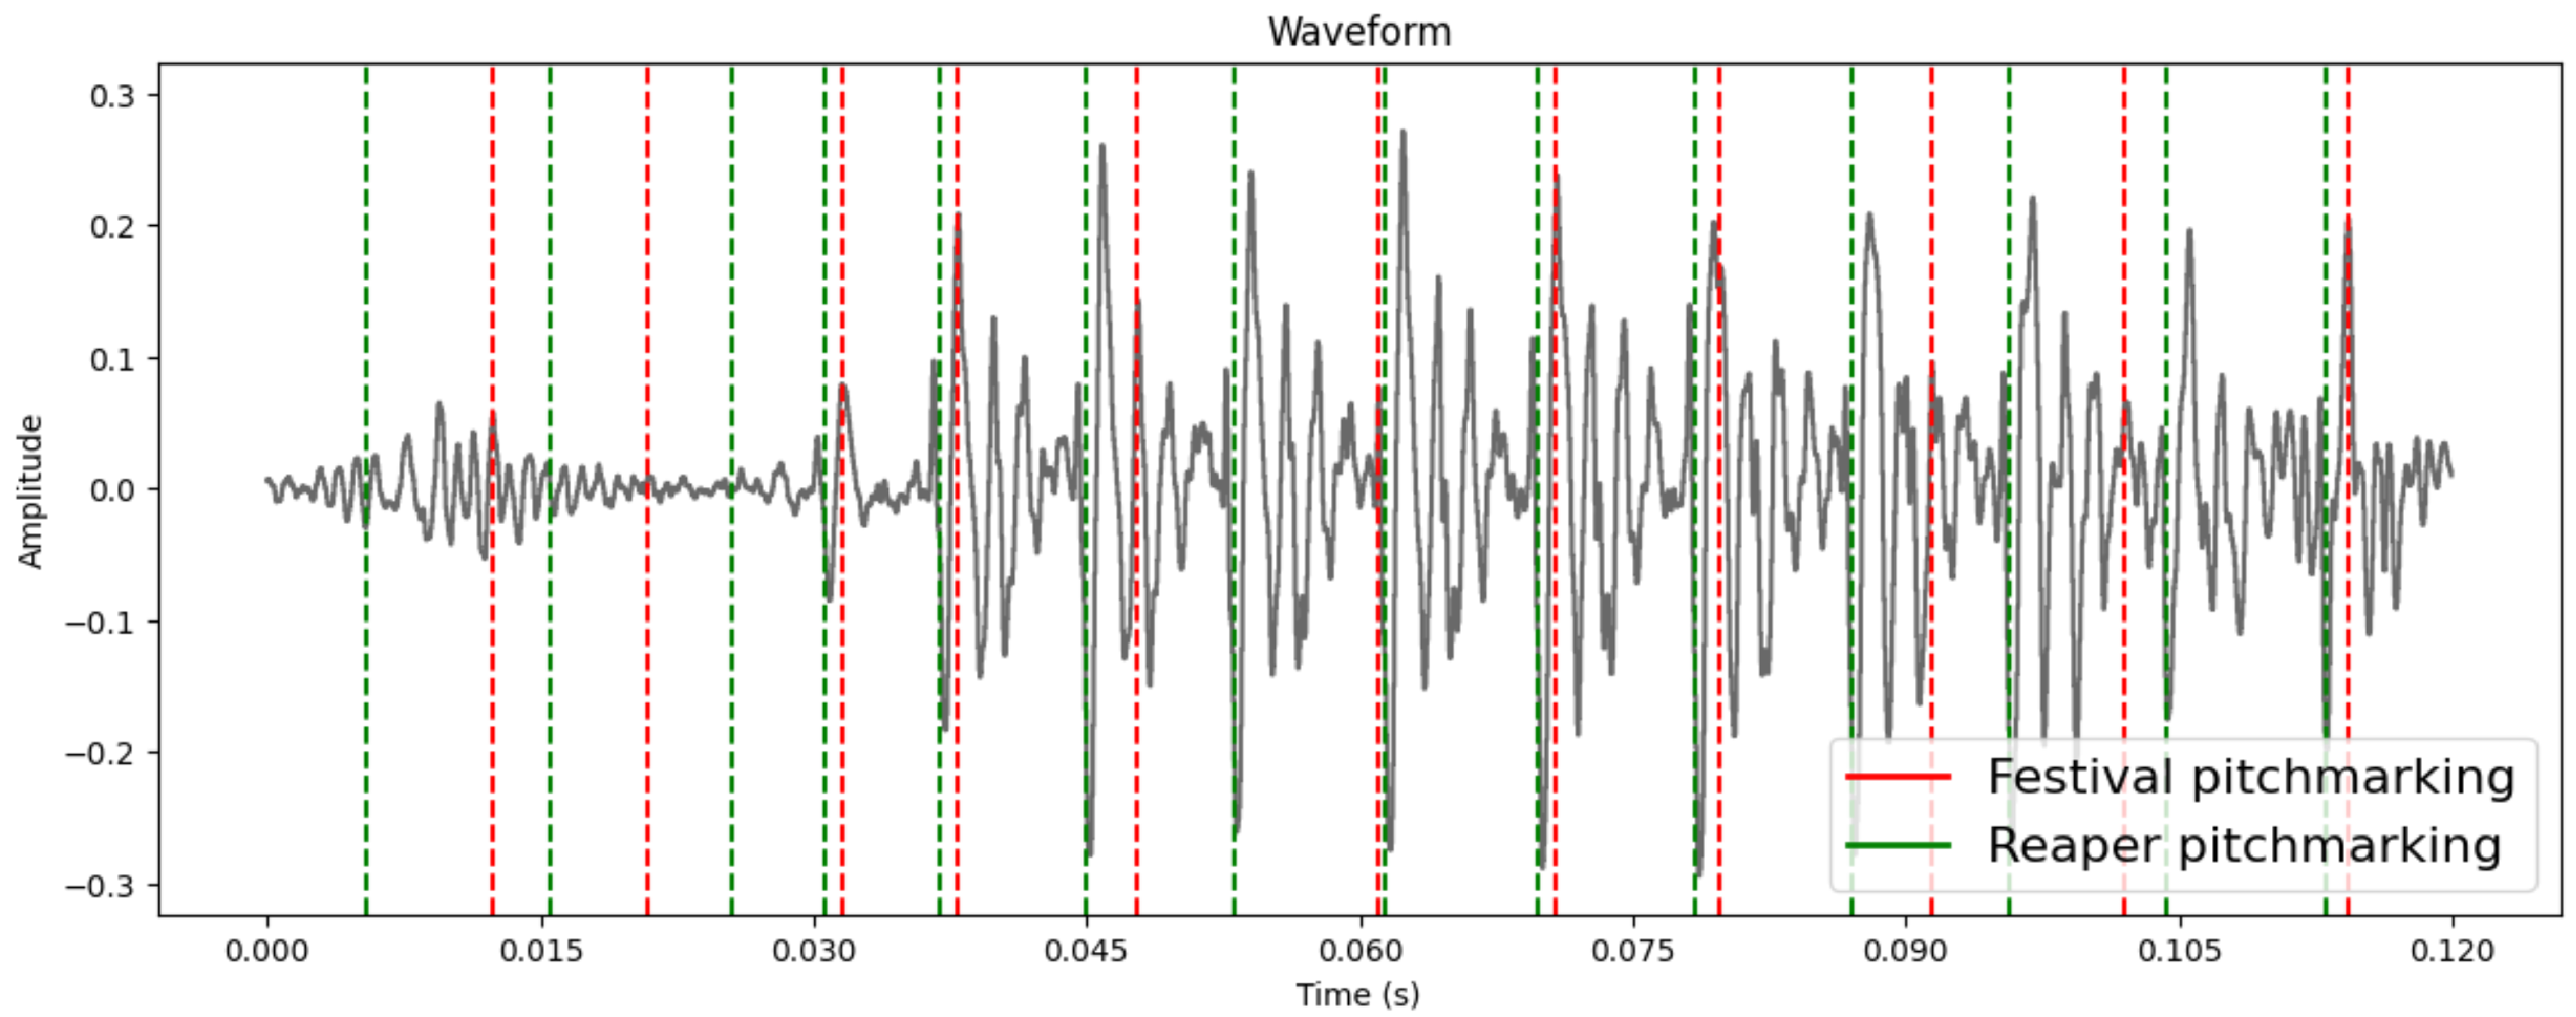
\includegraphics[width=\textwidth]{images/pm/pm.pdf}
    \caption{Visualization of pitch marking generated by Festival and REAPER.}
    \label{fig:pm}
\end{figure*}

The results of subjective evaluation of the naturalness of voices generated by Festival and \verb|REAPER|, \autoref{fig:bp} show the mean opinion scores (MOS) provided by listeners. We can observe that the human voice is consistently given the highest naturalness and the MOS score for \verb|REAPER| is slightly better than the Festival voice. We further do a significance testing, with Wilcoxon signed rank test \cite{Wilcoxon1945IndividualCB} at p-level $p < 0.05$. We get a Wilcoxon p-value of $0.4488 >> 0.05$ which demonstrates no significant differences between the MOS scores. This indicates that there is no perceivable difference in the naturalness between the two voices. We also perform an objective evaluation of the synthesized voices as shown in \autoref{table:pm_wer}. We find that the results are consistent with the MOS scores for naturalness, however, given that we only have 10 utterances for testing, the difference in WER is deemed insignificant. 


\begin{figure}[!htbp]
    \centering 
    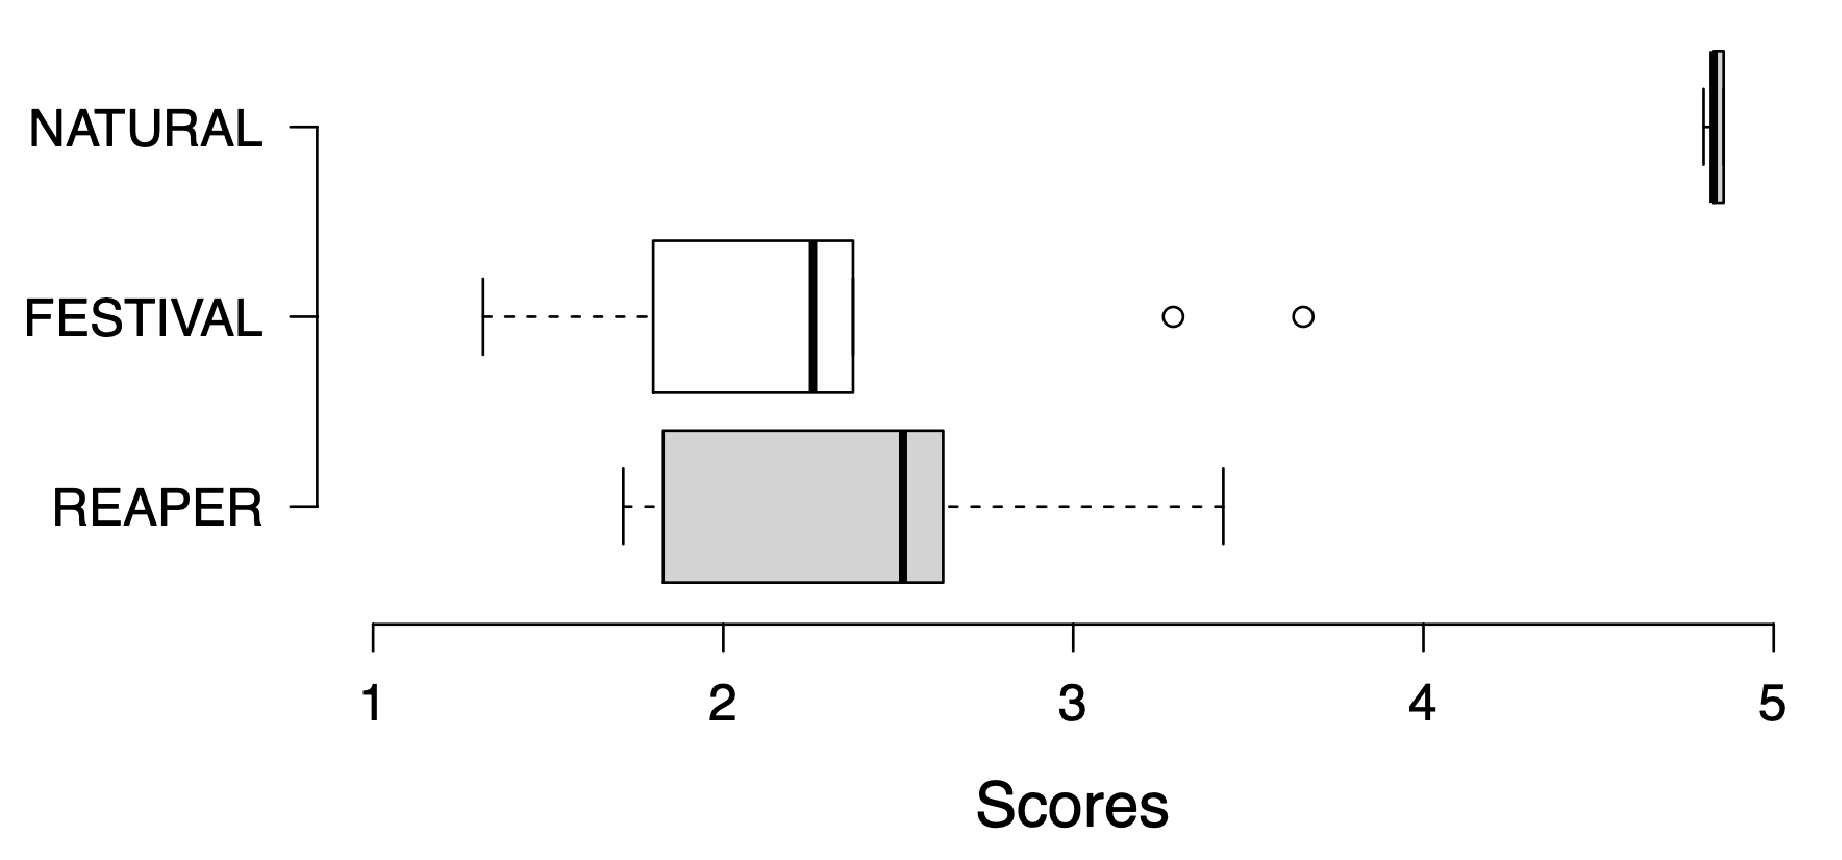
\includegraphics[width=0.5\textwidth]{images/pm/bp.pdf}
    \caption{Boxplot of MOS scores on the naturalness of synthesized voice using different pitch marking and F0 estimation algorithms}
    \label{fig:bp}
\end{figure}

\begin{table}
    \centering
    \begin{tabular*}{0.4\textwidth}{@{} l @{\extracolsep{\fill}} 
             d{5.0}d{5.0}d{5.0} @{}}
        \toprule
        \multicolumn{1}{c}{} 
        & \multicolumn{3}{c}{Voices} \\
        \cmidrule{2-4} 
        & \mc{REAPER} & \mc{Festival}  & \mc{Human}\\
        \midrule
        WER & $6.50\%$ & $7.10\%$ & $2.50\%$\\
        MOS & $2.45 ± 0.61$ & $2.30 ± 0.70$ & $4.83 ± 0.02$ \\
        \bottomrule
    \end{tabular*}
    \caption{Subjective and objective evaluation results for exploring the effect on naturalness and intelligibility of better pitch marking and F0 estimation algorithms}
    \label{table:pm_wer}

\end{table}

\subsection{Experiment 2: Domain adaptation of voice}

In this experiment, we would like to understand the effect of data size and domain of training data used to synthesize voice on the perception of naturalness by listeners. In corpus driven TTS system, domain adaptation is achieved by adding data from the target domain and synthesizing voice on the new data. \cite{domain_adaptation} Also, the synthesized speech on test data from a different domain is comparatively less natural and intelligible because of differences in prosodic requirements such as duration of words, intonation and also missing phones and diphones from the different domain.\cite{Clark2004Festival2}

We synthesized three voices \verb|Cooking (278)| , \verb|Cooking (600)| , \verb|Cooking+Arctic (1193)|. The voices \verb|Cooking (278)| and \verb|Cooking (600)| are from the dessert recipes domain with 278 and 600 utterances in the training script; 278 utterances provide $100\%$ diphone coverage and \verb|Cooking (600)| is synthesized with 322 additional data as discussed in Section \ref{section:auto_script_sel}. \verb|Cooking+Arctic (1193)| is synthesized with 600 utterances from dessert recipes and 593 utterances from CMU Arctic A \cite{Kominek2004TheCA} with data from out-of-copyright books from the Gutenberg Project; which means that additional data is out-of-domain. 

\autoref{fig:da} shows the results of subjective evaluation of comparative naturalness voices on the test utterances grouped by the domain of data. \autoref{table:da_wer} shows the results of the objective evaluation results of intelligibility.  Based on the results of listener preferences can conclude that for in-domain data the naturalness is in order \verb|Cooking (600)| $>$ \verb|Cooking (278)| $>$ \verb|Cooking+Arctic (1193)| and adding more data helps improve naturalness and intelligibility only when the additional data is from the same domain. We can also conclude that additional OOD data helps synthesized voice adapt better for out-of-domain data as listeners show a significantly higher preference for \verb|Cooking+Arctic (1193)| for OOD test utterances; however we cannot conclude that the resulting voice is of good quality as WER for OOD utterances is significantly higher than in-domain and near-in-domain cases as shown in \autoref{table:da_wer}, but comparatively lower than other voices.


% https://tex.stackexchange.com/a/211476
\begin{table}
    \begin{tabular*}{0.45\textwidth}{@{} l @{\extracolsep{\fill}} 
             d{4.0}d{4.0}d{4.0} @{}}
        \toprule
        \multicolumn{1}{c}{Voice} 
        & \multicolumn{3}{c}{Test Data Type (WER)} \\
        % & \multicolumn{2}{c}{$N = 3$}
        % & \multicolumn{2}{c@{}}{$N = 4$}\\  
        \cmidrule{2-4} 
        & \mc{In} & \mc{Near} & \mc{Out of}\\
        & \mc{Domain} & \mc{In Domain} & \mc{Domain}\\
        \midrule
        Cooking (278) & $6.50\%$ & $8.10\%$ &  $17.40\%$ \\
        Cooking (600) & $3.20\%$ & $5.40\%$ & $13.00\%$ \\
        Cooking+Arctic & $11.30\%$ &  $7.90\%$ &  $11.50\%$ \\ 
        \bottomrule
    \end{tabular*}
    \caption{Results for comparison of effect of data quantity and domain on intelligibility}
    \label{table:da_wer}
\end{table}


\begin{figure}[!t]
\centering
    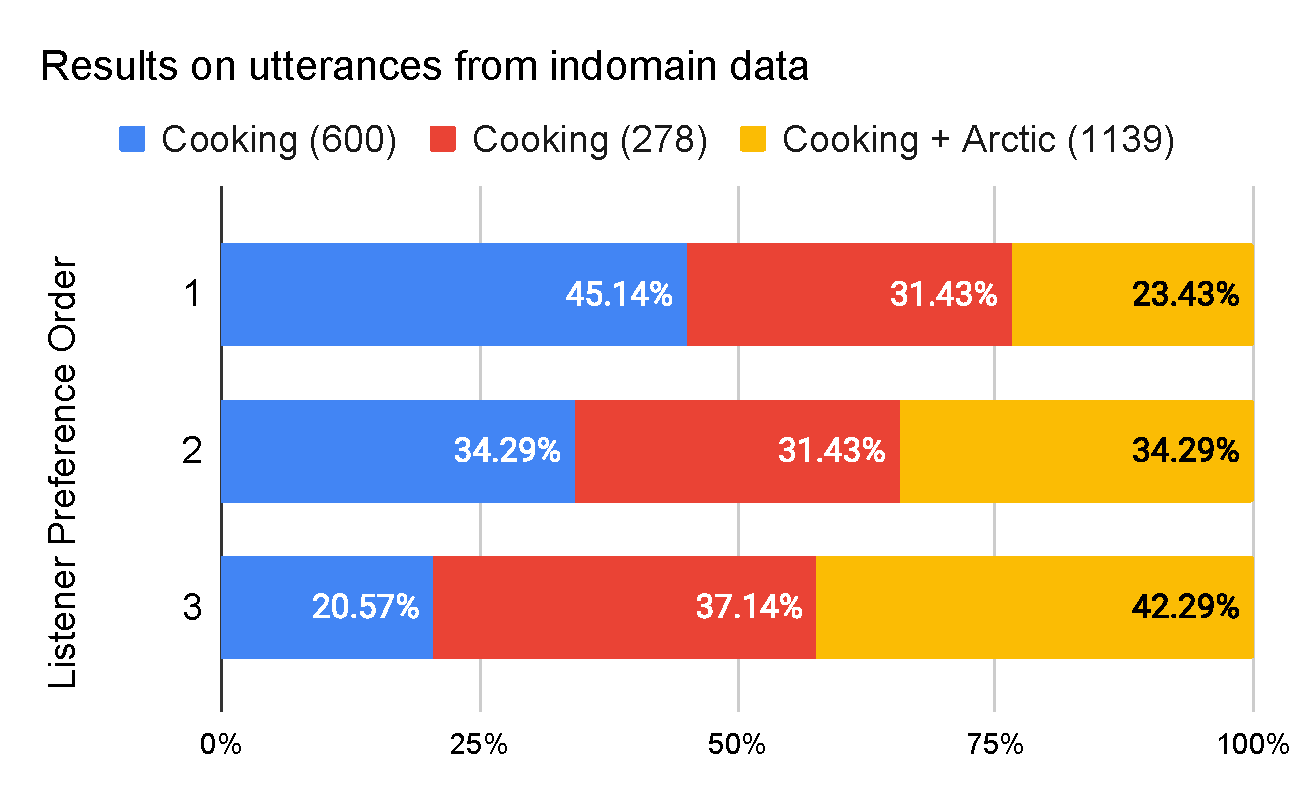
\includegraphics[width=0.95\columnwidth]{images/da/id.pdf}
    \includesvg[width=0.95\columnwidth]{images/da/nid.svg}
    \includesvg[width=0.95\columnwidth]{images/da/ood.svg}
\caption{Results of listener ranked preference of synthesized voice showing the effect of data quantity and domain on perceived naturalness. Lower ranks show higher preference.}
\label{fig:da}
\end{figure}

% \begin{figure}[!htbp]
%     \centering \includesvg[width=0.5\textwidth]{images/da/id.svg}
%     \caption{in domain}
%     \label{fig:da_id}
% \end{figure}

% \begin{figure}[!htbp]
%     \centering \includesvg[width=0.5\textwidth]{images/da/nid.svg}
%     \caption{near in domain}
%     \label{fig:da_nid}
% \end{figure}

% \begin{figure}[!htbp]
%     \centering \includesvg[width=0.5\textwidth]{images/da/ood.svg}
%     \caption{out of domain}
%     \label{fig:da_ood}
% \end{figure}





% \subsection{Experiment 3: Effective use of pronunciation dictionary}

% When the speaker's accent does not match the pronunciation dictionary, the TTS system may generate incorrect pronunciations, resulting in poor-sounding speech.
% For example, if the speaker has a British accent and the pronunciation dictionary is based on a General American accent, words such as "caught" will be pronounced differently. This will lead to poor alignment during the forced alignment step, which will result in unnatural speech.


% \begin{figure}[!htbp]
%     \centering \includesvg[width=0.5\textwidth]{images/pd/bf.svg}
%     \caption{out of domain}
%     \label{fig:da_ood}
% \end{figure}


% \begin{table}
%     \centering
%     \begin{tabular*}{0.3\textwidth}{@{} l @{\extracolsep{\fill}} 
%              d{2.0}d{2.0} @{}}
%         \toprule
%         \multicolumn{1}{c}{} 
%         & \multicolumn{2}{c}{Voices} \\
%         \cmidrule{2-3} 
%         & \mc{Cooking GAM} & \mc{ Cooking RPX} \\
%         \midrule
%         WER & $3.20\%$ & $4.80\%$ \\
%         \bottomrule
%     \end{tabular*}
%     \caption{Word error rate}
%     \label{fig:pd_wer}

% \end{table}




\section{Discussion and Conclusion}
\label{section:discussion_n_conclusion}
% In this report we explored the process of building a unit selection voice for text-to-speech synthesizer. The main focus was given to the waveform generator stage of the synthesis pipeline. We started with a discussion of an overview of unit selection synthesis and how such a well designed system could result in high quality voice with the prosodic properties of recorded domain data which is highly natural and intelligible. We discuss the major components for unit selection algorithm which consists of target construction which focuses on adding linguistic specification of the recorded units in the database. We then discuss target cost and join cost and how they are used withing the unit selection algorithm and how they impact the selection of candidate unit sequence. We conclude by discussing how to search for the best candidate unit sequence using Viterbi search and how waveform of the optimal unit sequence is combined to result in the most natural and intelligible synthesized speech.

% The voice we build focused on reading out dessert recipes in cooking domain. For building the unit selection voice we collected data by scraping websites. We then cleaned and normalized the data such that it is suitable for recoding purposes. A greedy algorithm which focuses on maximizing the diphone coverage for automatic script selection. We created a script of 600 utterances and recorded them along with CMU Arctic A data which were used for voice building purposes. Next, we discussed the process of recording speech, which included the recording setup and various processing step to ensure that the recorded speech is ready for voice building process. Automatic corpus segmentation which includes automatic labeling of the recorded speech by using forced alignment mode of HTK based HMM training, which leads to alignment of phone sequences of utterances and recorded speech which is then used for segmenting diphones to prepare the unit candidates for unit selection database. The process of building utterance structure to include linguistic features, duration information, pitch marking, F0, MFCC coefficients etc. and how they are used and their effect in unit selection algorithm is discussed. 

% Lastly, we design listening test and discussed the results of two experiments with the help of 39 volunteer who performed the listening tests. We design an experiment to understand the effect of perceived naturalness when using a more robust pitchmarking and pitch tracking algorithm \verb|REAPER| in comparison to Festivals algorithms for the same. We conducted subjective evaluation of naturalness of synthesized voices using mean opinion score and found that listeners gave a slightly higher mean score to \verb|REAPER| voice, however, significance testing shows that they preference is not significant. We also performed an objective evaluation using Whisper \cite{radford2022whisper} ASR system, and found that \verb|REAPER| voice has $0.60\%$ better WER, however given the size of our test utterances we concluded the difference to be insignificant. Second experiment, which were aimed at evaluating the effect of data quantity and data domain on domain adaptation on synthesized voices. We performed a listener preference testing by ranking of voices as part of subjective evaluation and ASR based automatic transcription objective test. We concluded that adding additional data from similar domain helps in improving in-domain and near-indomain naturalness and intelligibility, where voice synthesized using one-fourth data from in-domain performs better than voice-synthesized using the data which is out-of-domain.

% We can conclude by saying that unit-selection based TTS system is capable of building highly natural and intelligible synthesized voices with little effort. The quality of data both in terms of recording setup and phonetic coverage to ensure we have context sensitive diphone candidates could significantly improve the quality of synthesized voice. With a large enough unit selection database, we can synthesize voices which can cover most of the prosodic variation of any domain and we can result is very natural and intelligible speech with little processing of waveform during concatenation of candidate units when compared to other concatenative synthesis methods.

In this report, we investigated the process of building a unit selection voice for text-to-speech (TTS) synthesizers, with a primary focus on the waveform generator stage of the synthesis pipeline. We began with an overview of unit selection synthesis, discussing how a well-designed system could produce high-quality voices that are natural and intelligible. We examined the main components of the unit selection algorithm, including target construction, target cost, and join cost, and how they impact the selection of candidate unit sequences. We also discussed the Viterbi search for identifying the best candidate unit sequence and how the waveform of the optimal sequence is concatenated to result in natural and intelligible synthesized speech.

Our TTS system was designed to speak dessert recipes such that it sounds natural and intelligible to humans. We collected data by scraping websites, cleaned and normalized it for recording purposes, and employed a greedy algorithm for maximizing diphone coverage. We generated a script of 600 utterances and recorded them alongside CMU Arctic A data. We then detailed the speech recording process, including setup and processing steps. Automatic corpus segmentation, using forced alignment mode of HTK-based HMM training, aligned phone sequences of utterances and recorded speech, segmenting diphones to prepare candidate units for the unit selection database. We explored building utterance structures that include linguistic features, duration information, pitch marking, F0, MFCC coefficients, and their effects on the unit selection algorithm.

We designed listening tests and analyzed the results of two experiments with 39 non-expert listeners, of which $60\%$ are native English speakers. The first experiment evaluated perceived naturalness using the robust REAPER pitch marking and F0 estimation algorithm compared to Festival's algorithms. Subjective evaluation of naturalness using mean opinion scores revealed a slightly higher preference for the REAPER voice, but significance testing showed no significant preference. Objective evaluation with the Whisper ASR system found a $0.60\%$ better WER for the REAPER voice, but given the test utterances' size, the difference was deemed insignificant. The second experiment assessed the effect of data quantity and domain on synthesized voices' domain adaptation. Listener preference testing for naturalness by ranking of voices and ASR-based automatic transcription was used for subjective and objective evaluations, respectively. We concluded that additional in-domain data improved in-domain and near in-domain naturalness and intelligibility, where voices synthesised with one-fourth of in-domain data performed better than those using additional out-of-domain data.

In conclusion, unit-selection-based TTS systems can create natural and intelligible synthesized voices with minimal effort. Ensuring data quality in terms of recording setup and phonetic coverage for context-sensitive diphone candidates can significantly enhance synthesized voice quality. With a large enough unit selection database, we can generate voices covering a majority of prosodic variations within the domain, resulting in natural and intelligible speech with minimal waveform processing during candidate unit concatenation compared to other concatenative synthesis methods.



% arctic A - 41 minutes
% cooking - 1 hour 33 minutes
% \subsection{Challenges Encountered and Solutions}
% \subsection{Limitations of the Developed Voice}
% \subsection{Potential Improvements and Future Work}

% \subsection{Summary of Findings}
% \subsection{Implications and Contributions}
% \subsection{Final Remarks}



\bibliographystyle{IEEEtran}
\bibliography{bibliography.bib}

\end{document}
